\documentclass[11pt]{article}
\usepackage{amsmath}
%\usepackage{extsizes}
\usepackage{amsmath,amssymb}
%\usepackage{omegavn,ocmrvn}
%\usepackage[utf8x]{inputenc}
\usepackage[utf8]{vietnam}

\usepackage{longtable}
\usepackage{answers}
\usepackage{graphicx}
\usepackage{array}
\usepackage{pifont}
\usepackage{picinpar}
\usepackage{enumerate}
\usepackage[top=3.0cm, bottom=3.5cm, left=3.5cm, right=2.5cm] {geometry}
\usepackage{hyperref}


\newtheorem{bt}{Câu}
\newcommand{\RR}{\mathbb R}
\Newassociation{sol}{Solution}{ans}
\newtheorem{ex}{Câu}
\renewcommand{\solutionstyle}[1]{\textbf{ #1}.}


\begin{document}
% \noindent
\begin{tabular*}
{\linewidth}{c>{\centering\hspace{0pt}} p{.7\textwidth}}
Trường ĐHKHTN, ĐHQGHN & {\bf Học Kỳ 1 (2020-2021)}
\tabularnewline
K63 TTƯD - Thầy Hà Phi & {\bf Bài Tập Giải Tích Số \\ Giải số hệ phi tuyến - Bài tập ứng dụng}
\tabularnewline
\rule{1in}{1pt}  \small  & \rule{2in}{1pt} %(Due date:)
\tabularnewline

%  \tabularnewline
%  &(Đề thi có 1 trang)
\end{tabular*}
%
% \Opensolutionfile{ans}[ans1]

\begin{bt} % Exercise 15, Kiusalass p.167
Các tần số riêng của dầm công-xôn (console) \\ (\verb|https://www.engineeringtoolbox.com/cantilever-beams-d_1848.html|) \\
liên quan đến các nghiệm $\beta_i$ của phương trình tần số $f(\beta) = cosh \beta cos \beta + 1 = 0$, trong đó
\hskip 4cm
\begin{tabular}{lll}
& $\beta_i^4 = (2 \pi f_i)^2 \ \dfrac{mL^3}{E \ I}$, \quad & $f_i$ là tần số tự nhiên thứ i (cps) \\
& $m$ là khối lượng của dầm, \quad & L là chiều dài thanh dầm \\
& E là mô đun đàn hồi (biến dạng), \quad & I là mômen quán tính của mặt cắt ngang.
\end{tabular}
%

\noindent Xác định hai tần số thấp nhất của một dầm thép 0,9 m dài, có mặt cắt ngang hình chữ nhật, rộng 25 mm và cao 2,5 mm. Khối lượng riêng của thép là
$kg/m^3$ và E = 200 GPa.
\end{bt}

\begin{bt}  % Exercise 16, Kiusalass p.167
Một sợi dây cáp bị buông trùng như hình vẽ. Độ dài s và độ võng h của nó có liên quan đến khoảng cách L thông qua phương trình
\begin{equation}
s = \dfrac{2}{\lambda} \sinh \dfrac{\lambda \ L}{2}, \quad 
h = \dfrac{1}{\lambda} \left( \cosh\dfrac{\lambda \ L}{2} - 1 \right)
\end{equation}
trong đó $\lambda = w_0/T_0$, với $w_0$ là trọng lượng của sợi cáp trên mỗi đơn vị độ dài, $T_0$ là độ căng của cáp tại O. Tính $s$ với $L = 160$ m và $h = 15$ m.
\begin{figure}[!h]
	\centering
	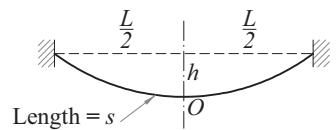
\includegraphics[width=0.4\linewidth]{suspended_cable}
	\caption{Exercise 16, Kiusalass p.167}
	\label{fig:suspendedcable}
\end{figure}
\end{bt}


\begin{bt}  % Exercise 17, Kiusalass p.167
Cột nhôm W $310 \times 202$ (mặt bích rộng) chịu tải trọng lệch tâm trục P như hình vẽ. Áp suất nén lớn nhất trong cột được cho bởi \textbf{công thức dây cung}
%
\begin{equation}
\sigma_{max} = \tilde{\sigma} \left[ 1 + \dfrac{e c}{r^2} \ \sec \left( \dfrac{L}{2r} \ \sqrt{\dfrac{\tilde{\sigma}}{E}}\right) \right] \ ,
\end{equation}
%
trong đó \\
\hskip .2cm
\begin{tabular}{lll}
& $\tilde{\sigma}$ = P/A là áp suất trung bình, & \\
& A=25800 $mm^2$ là diện tích mặt cắt ngang của cột, & \\
& e = 85 mm là độ lệch tâm của tải, \quad & c = 170 mm là nửa chiều sâu của cột, \\
& r= 142 mm là bán kính chuyển động của mặt cắt ngang, \quad & L là 7100 mm là chiều dài của cột, \\
& $E$ = 71 $\times 10^9$ Pa là môđun đàn hồi . &\\
\end{tabular}

\noindent Xác định tải trọng lớn nhất P mà cột có thể chịu được nếu áp suất lớn nhất không vượt quá $120 \times 10^6$ Pa.
%
\begin{figure}[h!]
	\centering
	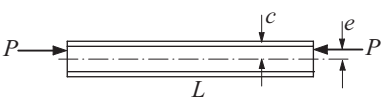
\includegraphics[width=0.4\linewidth]{aluminum_column.png}
	\caption{Exercise 17, Kiusalass p.167}
	\label{fig:aluminumcolumn}
\end{figure}
\end{bt}

\begin{bt}  % Exercise 18, Kiusalass p.168
	Phương trình Bernoulli’s cho dòng chất lỏng chảy qua một kênh mở với một vết lồi nhỏ là
	\begin{equation}
		\dfrac{Q^2}{2gb^2h^2_0 } + h_0 = \dfrac{Q^2}{2gb^2h^2} + h + H
	\end{equation}
	trong đó \\
	\begin{tabular}{ccc}
		$Q = 1.2 \ m^3/s$ & = &  vận tốc (khối) của dòng chất lỏng\\ 
		$g = 9.81 m/s^2$ & = &  gia tốc của lực hấp dẫn \\ 
		$b = 1.8$ m & = & độ rộng kênh \\ 
		$h_0 = 0.6$ m & = & mực nước ngược dòng \\
		$H = 0.075$ m & = & độ cao của vết lồi \\ 
		h & = & mức nước ở trên vết lồi \\ 
	\end{tabular}
	
	\noindent Hãy đi tính h. 
	%
	\begin{figure}[h!]
		\centering
		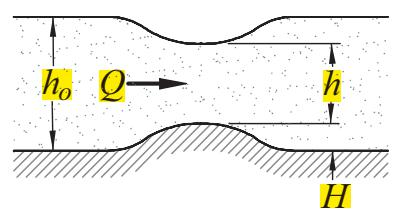
\includegraphics[width=0.4\linewidth]{open_channel}
		\caption{Exercise 18, Kiusalass p.168}
		\label{fig:openchannel}
	\end{figure}
\end{bt}

\newpage 

\begin{bt}  % Exercise 19, Kiusalass p.169
\verb|Exercise 19, Kiusalass p.169| \\	
Tốc độ v của tên lửa Saturn V khi bay thẳng đứng gần bề mặt trái đất có thể được tính gần đúng bằng
\begin{equation}
v = u \ \ln \dfrac{M_0}{M_0 - m t} - gt
\end{equation}
trong đó \\
u = 2 510 m/s = vận tốc của khí thải so với tên lửa \\
M0 = 2,8 $\times$ 106 kg = khối lượng tên lửa khi cất cánh \\
m = 13,3 $\times$ 103 kg / s = tốc độ tiêu thụ nhiên liệu \\
g = 9,81 m / s2 = gia tốc trọng trường \\
t = thời gian đo được từ khi cất cánh \\
Xác định thời điểm tên lửa đạt vận tốc âm thanh (335 m / s).
\end{bt}

\begin{bt}
Thùng dầu hình trụ có bán kính r và chiều dài L được đổ đầy đến độ sâu h. Kết quả
khối lượng dầu trong thùng là
\[
V = r^2L \Big( \phi - \left(1 - \dfrac{h}{r}\right) sin \phi \Big)
\]
trong đó $\phi = arcos\left(1 - \dfrac{h}{r}\right)$. Nếu bể đầy 3/4, hãy xác định tỉ số $h/r$.

\begin{figure}[h!]
	\centering
	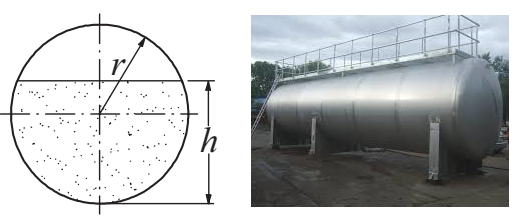
\includegraphics[width=0.7\linewidth]{oil_tank}
	\caption{}
	\label{fig:oiltank}
\end{figure}
\end{bt}

\pagebreak 

\begin{bt} % Exercise 27, Kiusalass p.171
Quỹ đạo của vệ tinh quay quanh trái đất là
\begin{equation*}
R =\dfrac{C}{1 + e \sin (\theta + \alpha)}
\end{equation*}
trong đó $(R, \theta)$ là tọa độ cực của vệ tinh, và $C$, $e$, và $\alpha$ là các hằng số ($e$ được gọi là độ lệch tâm của quỹ đạo). Nếu vệ tinh được quan sát tại
ba vị trí sau
\vskip .2cm
\begin{center}
\begin{tabular}{|l|l|l|l|}
\hline
$\theta$ & -30\ $^{\circ}$ & 0\ $^{\circ}$  & 30\ $^{\circ}$ \\ \hline
$R (km)$ & 6870 & 6728 & 6615 \\ \hline 
\end{tabular}
\end{center}
\vskip.2cm
Hãy xác định $R$ nhỏ nhất của quỹ đạo và giá trị tương ứng của $\theta$.
	\begin{figure}[!h]
	\centering
	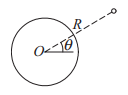
\includegraphics[scale = 1.2]{sateline}
	\caption{}
	\label{fig:sateline}
\end{figure}
\end{bt}

\begin{bt}
Và còn khá nhiều bài tập khác trong cùng Chương này của Kiusalass mà thầy không có thời gian để dịch nốt nhưng vẫn có thời gian để cho vào đề thi. 
\end{bt}
\centerline{———————————Hết——————————-}

\end{document}

\vspace{1cm}
\noindent{\bf Chú ý:} {\it Cán bộ coi thi không giải thích gì thêm}\\
\Closesolutionfile{ans}
\newpage
\begin{center}
{\LARGE{\bf ĐÁP ÁN}}
\end{center}

\begin{sol}
	\begin{figure}[h!]
		\centering
		\includegraphics[width=0.8\linewidth]{Solution1/Sol4_1.png}
		%\caption{}
		\label{fig:Sol4}
	\end{figure}
	Exercise 7: Convergence order is 3.	
\end{sol}

   
\end{document}



